% **************************************************************************** %
\chapter{Modellierung eines Photovoltaik-Systems}
\label{chap:models}
% **************************************************************************** %

Bevor  simuliert  werden  kann,  m\"ussen  die  daf\"ur  ben\"otigten  Modelle
vorhanden  sein. In diesem  Abschnitt wird  im \emph{bottom-up}-Verfahren  das
Modell eines Strangs  aus PV-Modulen mit Zuleitung  entwickelt. Es wird zuerst
das Modell einer Zelle definiert, aus dem anschliessend ein PV-Modul aufgebaut
wird.  Das Modell  des PV-Moduls wird dann wiederum benutzt,  einen Strang aus
Modulen zu modellieren.

Die    entwickelten     Modelle    werden    anschliessend     im    Abschnitt
\emph{\titleref{chap:simu}} in \code{LTspice}-Simulationen verwendet, um unsere
L\"osungsans\"atze zu untersuchen.

\emph{Konvention:} Doppelt unterstrichene Werte in Gleichungen sind Parameter,
welche in unser Model aufgenommen werden.

% ---------------------------------------------------------------------------- %
\section{Modellierung einer PV-Zelle}
\label{sec:simu:model:cell}
% ---------------------------------------------------------------------------- %

\begin{wrapfigure}{r}{65mm}
    \centering
    % Simple Single-Diode Model
\begin{circuitikz}
    \footnotesize
    \draw
    % Source to top terminal
    (0,0) to[current source,i=$I_{\mathrm{Ph}}$] (0,2) -- (2,2) to[R,l^=$R_{\mathrm{S}}$] (4,2) node[ocirc] {}

    % Open terminal at bottom
    (4,0) node[ocirc] {} -- (0,0)

    % Voltage arrow over open terminals
    (4,1.7) -- (4,0.3) node[currarrow,rotate=-90] {}
    (4,1) node[anchor=west] {$V_{\mathrm{offen}}$}

    % Parallel elements
    (1,0) to[empty diode,*-*,l_=$D$] (1,2)
    (2,0) to[R,*-*,l_=$R_{\mathrm{Sh}}$] (2,2)
    ;
\end{circuitikz}

    \caption[Eindiodenmodell PV-Zelle]{%
        Eindiodenmodell  einer  PV-Zelle  mit  Stromquelle  $I_{\mathrm{Ph}}$,
        Diode  $D$,  Shunt-Widerstand $R_{\mathrm{Sh}}$~  und  Seriewiderstand
        $R_{\mathrm{S}}$.%
    }
    \label{fig:pvcell:1diode}
\end{wrapfigure}

Das Modell  einer idealien  Photovoltaikzelle ist  eine Stromquelle  mit einer
parallel geschalteten Diode. Da PV-Zellen in Realit\"at nicht ideal sind, wird
das einfachste Ersatzschaltbild einer PV-Zelle \"ublicherweise durch einen zur
Stromquelle parallel geschalteten Shunt-Widerstand $R_{\mathrm{Sh}}$ und einen
Seriewiderstand $R_{\mathrm{S}}$ erg\"anzt; das resultierende Ersatzschaltbild
ist in Abbildung \ref{fig:pvcell:1diode} dargestellt.

Die Genauigkeit  dieses Eindiodenmodells  ist jedoch h\"aufig  nicht besonders
gut  \cite{pvcell:phang}  \cite{pvcell:masmoudi}   (besonders  bei  niederigen
Beleuchtungsgraden),   weshalb   wir   hier  ein   Zweidiodenmodell   benutzen
werden. Eine  der  beiden  Dioden   modelliert  dabei  den  S\"attigungsstrom,
welcher von  Diffusionsprozessen verursacht wird, die  zweite Diode modelliert
den  S\"attigungsstrom,  welcher  von Rekombinationseffekten  verursacht  wird
\cite{pvcell:masmoudi}.

Zur Herleitung der Modellparamater existieren verschiedene Verfahren. Man kann
beispielsweise eine  PV-Zelle im Labor  ausmessen und die  Modellparameter aus
diesen  Messergebnissen  ableiten.   Dies  ist jedoch  nicht  immer  praktisch
realisierbar, da man allenfalls kein Testexemplar zur Verf\"ugung hat.  Sollen
bei  der  Messung  noch Fertigungstoleranzen  der  PV-Zellen  ber\"ucksichtigt
werden,  steigt der  experimentelle  (und  finanzielle) Aufwand  zus\"atzlich,
da  man  mehrere Exemplare  kaufen  und  ausmessen muss. Auch  die  Auswertung
erfordert mehr Arbeit, wenn  man mittels statistischer Methoden verl\"assliche
Schlussfolgerungen ziehen k\"onnen will.

Alternativ   kann   man   auch   versuchen,  die   Modellparameter   aus   dem
Datenblatt  einer  PV-Zelle  herzuleiten. Dies  bietet  zwei  haupts\"achliche
Vorteile: Einerseits  entfallen  aufw\"andige  Messungen   und  der  Kauf  von
Testexemplaren, andererseits ist davon auszugehen, dass der Hersteller mehrere
Exemplare ausgemessen hat  und typische Angaben in  den Datenbl\"atten gemacht
werden.  Es setzt jedoch voraus,  dass man den Herstellerangaben einigermassen
vertraut;  Sicherheit  ist  letztendlich  nur  durch  eigene  Verifikation  zu
erlangen.

Das Herleiten der Modellparameter aus den Herstellerangaben ist nicht trivial;
es wird deshalb  an dieser Stelle ein Modell  einer kommerziell erh\"altlichen
PV-Zelle  (M5SF-2 von  \emph{JA Solar})  als Grundlage  verwendet, welches  in
\cite{pvcell:masmoudi} hergeleitet und verifiziert worden ist.

\"Ublicherweise wird  bei PV-Zellen  nur das  Gleichstromverhalten untersucht;
das Verhalten  unter Wechselstrom interessiert meistens  nicht. Da das Signal,
welches  in  diesem  Projekt  auf die  DC-Leitung  aufmoduliert  wird,  jedoch
Wechselstrom ist,  sollte das  Wechselstromverhalten von PV-Zellen  in unseren
Simulationen ber\"ucksichtigt werden.

Das  Zweidiodenmodell  aus  \cite{pvcell:masmoudi}  wird  deshalb  in  unseren
Simulationen noch durch eine parallele Kapazit\"at erg\"anzt, wie in Abbildung
\ref{fig:circuit:solarCell} gezeigt.

\begin{figure}[h!tb]
    \centering
    % Parametrized version, can be put at coordinates x and y
%
%\newcommand{\CTSolarCell}[2]{%
%    % Source to top terminal
%    (0+#1,0+#2) to[current source,i=$I_{\mathrm{Zelle}}$] (0+#1,4+#2) -- (5+#1,4+#2) to[R,l^=$R_{\mathrm{S}}$] (10+#1,4+#2) node[circ] {}
%
%    % Open terminal at bottom
%    (10+#1,0+#2) node[circ] {} -- (0+#1,0+#2)
%
%    % Voltage arrow over open terminals
%    %(10+#1,3.7+#2) -- (10+#1,0.3+#2) node[currarrow,rotate=-90] {}
%    %(10+#1,2+#2) node[anchor=west] {$V_{\mathrm{offen}}$}
%
%    % Parallel elements
%    (1.5+#1,4+#2) to[empty diode,*-*,l_=$D$] (1.5+#1,0+#2)
%    (3+#1,4+#2) to[C,*-*,l_=$C$] (3+#1,0+#2)
%    (4.5+#1,4+#2) to[R,*-*,l_=$R_{\mathrm{P}}$] (4.5+#1,0+#2)%
%}


% Single Diode
%\begin{circuitikz}
%    \draw
%    % Source to top terminal
%    (0,0) to[current source,i=$I_{\mathrm{Zelle}}$] (0,3) -- (5,3) to[R,l^=$R_{\mathrm{S}}$] (8,3) node[ocirc] {}
%
%    % Open terminal at bottom
%    (8,0) node[ocirc] {} -- (0,0)
%
%    % Voltage arrow over open terminals
%    (8,2.7) -- (8,0.3) node[currarrow,rotate=-90] {}
%    (8,1.5) node[anchor=west] {$V_{\mathrm{offen}}$}
%
%    % Parallel elements
%    (1.5,3) to[empty diode,*-*,l_=$D$] (1.5,0)
%    (3,3) to[C,*-*,l_=$C$] (3,0)
%    (4.5,3) to[R,*-*,l_=$R_{\mathrm{P}}$] (4.5,0)
%    ;
%\end{circuitikz}

% Two Diodes
\begin{circuitikz}
    \draw
    % Source to top terminal
    (0,0) to[current source,i=$I_{\mathrm{Ph}}$] (0,3) -- (7.5,3) to[R,l^=$R_{\mathrm{S}}$] (11,3) node[ocirc] {}

    % Open terminal at bottom
    (11,0) node[ocirc] {} -- (0,0)

    % Voltage arrow over open terminals
    (11,2.7) -- (11,0.3) node[currarrow,rotate=-90] {}
    (11,1.5) node[anchor=west] {$V_{\mathrm{offen}}$}

    % Parallel elements
    (2,3) to[empty diode,*-*,l_=$D_{\mathrm{Diff}}$] (2,0)
    (4.5,3) to[empty diode,*-*,l_=$D_{\mathrm{Rekomb}}$] (4.5,0)
    (6,3) to[C,*-*,l_=$C$] (6,0)
    (7.5,3) to[R,*-*,l_=$R_{\mathrm{Sh}}$] (7.5,0)
    ;
\end{circuitikz}

    \caption[Zweidiodenmodell PV-Zelle mit zus\"atzlicher Kapazit\"at]{%
        Schaltschema    zur    Modellierung    einer    Solarzelle    gem\"ass
        Zweidiodenmodell  mit  zus\"atzlicher  Kapazit\"at. Die  zugeh\"origen
        Modellparameter    sind    in    Tabelle    \ref{tab:solarCell:params}
        aufgelistet.%
    }
    \label{fig:circuit:solarCell}
\end{figure}

Die   Gr\"ossenordnung   dieser   Kapazit\"at   kann   stark   variieren   und
wird   unter  anderem   vom   Diodenmaterial,  der   Diodenspannung  und   der
Diodentemperatur   beeinflusst. Basierend    auf   \cite{capacitance:hegedus},
\cite{capacitance:mandal}     und      \cite{capacitance:mauk}     soll     an
dieser    Stelle   eine    fl\"achennormierte    Kapazit\"at    von   $C'    =
\SI{20}{\nano\farad\per\centi\meter\squared}$    verwendet   werden. Die    in
\cite{pvcell:masmoudi}    verwendete    Zelle    hat   eine    Gr\"osse    von
$\SI{125}{\milli\meter}    \times     \SI{125}{\milli\meter}$    (allf\"allige
abgeschnittene  Ecken, wie  sie in  Abbildung \ref{fig:pvcell:front}  zu sehen
sind,  werden  vernachl\"assigt),  womit  die  Kapazit\"at  einer  Zelle  sich
berechnet zu:

\begin{equation}
    \label{eq:capa:jac}
    C_{\mathrm{Zelle}}
    = A_{\mathrm{Zelle}} \cdot C'
    = \left( \SI{125}{\milli\meter} \right)^4 \cdot \SI{20}{\nano\farad\per\centi\meter\squared}
    = \underline{\underline{\SI{3.125}{\micro\farad}}}
\end{equation}

Somit  sind das  Ersatzschaltbild  und die  zugeh\"origen Parameter  bestimmt;
die  Ergebnisse  sind  in Abbildung  \ref{fig:circuit:solarCell}  und  Tabelle
\ref{tab:solarCell:params} abgebildet respektive aufgelistet.

\vspace*{6em}
\begin{table}[h!t]
    \centering
    \caption{\"Ubersicht Modellparameter f\"ur Solarzelle aus Abbildung \ref{fig:circuit:solarCell}}
    \label{tab:solarCell:params}
    \begin{tabular}{llrp{20mm}}
        \toprule
        Parameter                              & Symbol                  & Wert                       & Quelle                 \\
        \midrule
        Diodenstrom (\emph{Photo Current})     & $I_{\mathrm{Ph}}$       & \SI{5.889}{\ampere}        & \cite{pvcell:masmoudi} \\
        S\"attigungsstrom Diffusionsdiode      & $I_{\mathrm{S,Diff}}$   & \SI{794.06}{\pico\ampere}  & \cite{pvcell:masmoudi} \\
        S\"attigungsstrom Rekombinationsdiode  & $I_{\mathrm{S,Rekomb}}$ & \SI{5.0762}{\micro\ampere} & \cite{pvcell:masmoudi} \\
        Idealit\"atsfaktor Diffusionsdiode     & $n_{\mathrm{Diff}}$     & \num{1}                    & \cite{pvcell:masmoudi} \\
        Idealit\"atsfaktor Rekombinationsdiode & $n_{\mathrm{Rekomb}}$   & \num{2}                    & \cite{pvcell:masmoudi} \\
        Seriewiderstand                        & $R_{\mathrm{S}}$        & \SI{1.71}{\milli\ohm}      & \cite{pvcell:masmoudi} \\
        Shunt-Widerstand                       & $R_{\mathrm{Sh}}$       & \SI{59.23}{\ohm}           & \cite{pvcell:masmoudi} \\
        Kapazit\"at                            & $C$                     & \SI{3.125}{\micro\farad}   & \cite{capacitance:hegedus}, \cite{capacitance:mandal}, \cite{capacitance:mauk}, Gl. \ref{eq:capa:jac} \\
        Kantenl\"ange                          & $s$                     & \SI{125}{\milli\meter}     & \cite{pvcell:masmoudi} \\
        \bottomrule
    \end{tabular}
\end{table}

% ---------------------------------------------------------------------------- %
\clearpage
\section{Modellierung eines PV-Moduls}
\label{sec:simu:model:module}
% ---------------------------------------------------------------------------- %


Das  im   obigen  Abschnitt   hergeleitete  PV-Zellen-Modell  wird   nun  dazu
verwendet,   ein    Modell   f\"ur   ein   PV-Modul    aufzubauen. In   Anhang
\ref{app:commercial:modules}  auf Seite  \pageref{app:commercial:modules} sind
zum  Vergleich die  Daten  einiger kommerzieller  PV-Module mit  verschiedenen
Zellenkonfigurationen aufgelistet.

Es     wird    ein     PV-Modul     aus    72     in    Serie     angeordneten
Zellen    gew\"ahlt     und    implementiert. Es    wird     ebenfalls    eine
Freilaufdiode    parallel    zu     jedem    Modul    geschaltet,    basierend
auf     den      in     Abbildungen     \ref{fig:simu:iv-curves:array:generic}
\ref{fig:simu:iv-curves:array:generic:bypass}   gezeigten  Effekten   und  den
zugeh\"origen Anmerkungen.

\begin{wrapfigure}{l}{50mm}
    \centering
    \begin{tikzpicture}
    \begin{scope}[x={(0mm,50mm)},y={(0mm,-80mm)},line width=1pt,cap=round]

        \node[anchor=north west,inner sep=0pt] at (0,0) {%
            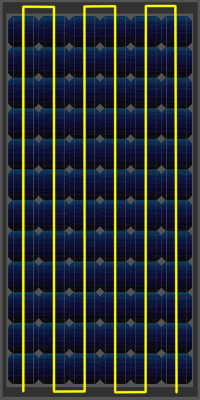
\includegraphics[width=40mm,height=80mm]{images/solar-facility/pvmodule-wiring.jpeg}
        };

        % Horizontal Measurement (Wires)
        % ==============================

        % Horizontal measurement between wires
        \draw (5mm,0mm) -- (5mm,4mm); % Vertical line
        \draw (11mm,0mm) -- (11mm,4mm);   % Vertical line

        % Measurement arrow
        \draw[-latex] (4mm,2mm) -- (5mm,2mm);
        \draw[-] (4mm,2mm) -- (31.5mm,2mm);
        \draw[latex-] (11mm,2mm) -- (12mm,2mm);

        % Measurment
        \node[anchor=west] at (12mm,3.75mm) {\small$d = \SI{127}{\milli\meter}$};


        % Vertical measurement (Wires)
        % ============================
        \draw (4mm,-1.5mm) -- (-4mm,-1.5mm); % horizontal line
        \draw (4mm,-78.5mm) -- (-4mm,-78.5mm); % horizontal line

        \draw[latex-latex] (-2mm,-1.5mm) -- (-2mm,-78.5mm); % measurement line

        % Measurement
        \node[rotate=90] at (-3.75mm,-38.5mm) {\small$l = \SI{1550}{\milli\meter}$};

        \node at (5mm,-82.5mm) {\small 1};
        \node at (11mm,-82.5mm) {\small 2};
        \node at (17mm,-82.5mm) {\small 3};
        \node at (23mm,-82.5mm) {\small 3};
        \node at (29mm,-82.5mm) {\small 2};
        \node at (35.5mm,-82.5mm) {\small 1};
    \end{scope}
\end{tikzpicture}


    \caption[PV-Modul, Modell f\"ur den Strompfad]{
        Solarmodul  gem\"ass Abbildung  \ref{fig:pvmodule} mit  Stromleitungen
        und  L\"angen   zur  Verbindung   der  Zellen. Die   Nummerierung  der
        Leiterbahnen   entspricht    der   Nummerierung    der   Koeffizienten
        in   Gleichungen   \ref{eq:rosa:a1}    bis   \ref{eq:rosa:a3}   (Seite
        \pageref{eq:rosa:a1}).%
    }
    \label{fig:pvmodule:wiring}
    \vspace*{-3em}
\end{wrapfigure}

Der  Pfad, den  der Strom  in  einem Modul  zur\"ucklegt, kann  je nach  Modul
mehrere Meter L\"ange  erreichen.  Dieser Effekt wird in  unserem Modell durch
eine Stromleitung modelliert, die \"uber  alle Zellen geht. In Realit\"at sind
die Leiter, welche die Zellen miteinander verbinden, ziemlich kurz (angenommen
die Zellen werden  von Kante zu Kante verbunden), aber  da der Strompfad durch
die ganze Zelle geht, wird der gesamte Strompfad in underem Modell vereinfacht
als eine lange Leitung dargestellt.

Zwischen   diesen   parallelen    Leiterbahnen   ergeben   sich   parasit\"are
Induktivit\"aten, die  im Folgenden  bestimmt und  in unser  Modell integriert
werden.  Die  angenommene Form und  die Abmessungen der  internen Stromleitung
sind  in  Abbildung   \ref{fig:pvmodule:wiring}  dargestellt. Die  Abmessungen
basieren auf folgenden Annahmen:

\begin{itemize}
    \tightlist
    \item
        Kantenl\"ange einer Zelle: \SI{125}{\milli\meter}
    \item
        Abstand zwischen zwei Modulen: \SI{2}{\milli\meter}
    \item
        \"Uberhang      am      oberen      und     unteren      Ende      des
        Moduls: \SI{14}{\milli\meter}
    \item
        Der Abstand zweier Leiterbahnen ist somit \SI{127}{\milli\meter} und
    \item
        die     L\"ange     einer     Leiterbahn     summiert     sich     auf
        \SI{1550}{\milli\meter}.
\end{itemize}


Zur  Berechnung  der  parasit\"aren  Induktivit\"at wird  \emph{The  Self  and
Mutual  Inductances  of Linear  Conductors}  von  Edward B. Rosa  herangezogen
\cite{ref:inductance:rosa}. Darin  wird   unter  anderem   die  Induktivit\"at
einer   Leiterkonfiguration  wie   sie  in   unserem  Modul   angenommen  wird
(Abbildung  \ref{fig:pvmodule:wiring}) bestimmt. Die  zugeh\"orige Formel  ist
in  Gleichung  \ref{eq:rosa:snake}  gegeben\footnotemark.
\footnotetext{%
    Die  Formeln  in   \cite{ref:inductance:rosa}  sind  im  \emph{CKG}-System
    (Centimeter,    Kilogramm,    Sekunden)     notiert,    f\"ur    Gleichung
    \ref{eq:rosa:snake} ist die Gleichung von  Rosa auf das SI-System normiert
    worden.%
}

\noindent Der  Wert f\"ur die Selbstinduktivit\"at  der verschiedenen Dr\"ahte
ist nicht  identisch; dies wird im  Summand $A_{\mathrm{i}}$ ber\"ucksichtigt,
der abh\"angt von der Anzahl  paralleler Leiterbahnen und ihrer Lage innerhalb
der  Leiteranordnung. F\"ur \num{6}  parallele Leiterbahnen  ergeben sich  die
Werte aus Gleichungen \ref{eq:rosa:a1}, \ref{eq:rosa:a2} und \ref{eq:rosa:a3}.


\begin{alignat}{2}
    \label{eq:rosa:snake}
    L &= \frac{\mu_{\mathrm{0}} \cdot l}{2 \cdot \pi}
    \cdot
    \left[
        \ln\left(
            \frac{d}{\rho}
        \right)
        + \frac{1}{4}
        - A_{\mathrm{i}}
    \right] & \quad \text{Selbstinduktivit\"at eines Leiters}
    \\
    \label{eq:rosa:a1}
    A_{\mathrm{1}} &= -\ln\left(\frac{15}{8}\right) & \text{\"ausserste Leiterbahnen} \\
    \label{eq:rosa:a2}
    A_{\mathrm{2}} &= \ln\left(\frac{16}{5}\right)  & \text{Leiterbahnen Nr. 2} \\
    \label{eq:rosa:a3}
    A_{\mathrm{3}} &= \ln\left(\frac{4}{3}\right)   & \text{Leiterbahnen Nr. 3, Mitte}
\end{alignat}

\begin{conditions}
    d              & Abstand zwischen zwei Leiterbahnen \\
    \rho           & Radius des Leiters \\
    A_{\mathrm{i}} & Korrektursummand f\"ur Leiterposition gem\"ass Abbildung \ref{fig:pvmodule:wiring} \\
\end{conditions}

Somit kann f\"ur  jeder Teil der Leitung in einem  Modul dessen Induktivit\"at
berechnet  werden. Diese  werden  anschliessend summiert  (Serieschaltung  von
Induktivit\"aten) und  als Gesamtinduktivit\"at  eines Moduls in  unser Modell
integriert.

Es   wird  von   einem   Leiterquerschnitt  von   \SI{4}{\milli\meter\squared}
ausgegangen,  was  einen   Leiterradius  $\rho$  von  \SI{1.128}{\milli\meter}
ergibt.

Die  Induktivit\"aten der  Leiterbahnen  innerhalb des  Moduls k\"onnen  somit
bestimmt werden:

\begin{alignat}{2}
    L_{\mathrm{1}} &= \frac{\mu_{\mathrm{0}} \cdot l}{2 \cdot \pi}
    \cdot
    \left[
        \ln\left(
            \frac{d}{\rho}
        \right)
        + \frac{1}{4}
        - A_{\mathrm{1}}
    \right]
    & = \SI{1.737}{\micro\henry} \\
    L_{\mathrm{2}} &= \frac{\mu_{\mathrm{0}} \cdot l}{2 \cdot \pi}
    \cdot
    \left[
        \ln\left(
            \frac{d}{\rho}
        \right)
        + \frac{1}{4}
        - A_{\mathrm{2}}
    \right]
    & = \SI{1.181}{\micro\henry} \\
    L_{\mathrm{3}} &= \frac{\mu_{\mathrm{0}} \cdot l}{2 \cdot \pi}
    \cdot
    \left[
        \ln\left(
            \frac{d}{\rho}
        \right)
        + \frac{1}{4}
        - A_{\mathrm{3}}
    \right]
    & = \SI{1.453}{\micro\henry}
\end{alignat}

\begin{conditions}
    \mu_{\mathrm{0}} = 4 \cdot \pi \cdot 10^{-7} & magnetische Permeabilit\"at des Vakuums \\
    l                = \SI{1550}{\milli\meter}   & L\"ange einer Leiterbahn                \\
    d                = \SI{127}{\milli\meter}    & Abstand zweier Leiterbahnen             \\
    \rho             = \SI{1.128}{\milli\meter}  & Radius des Leiters                      \\
    A_{\mathrm{1}}   =  -0.6286                  & Korrektursummand                        \\
    A_{\mathrm{2}}   =   1.1632                  & Korrektursummand                        \\
    A_{\mathrm{3}}   =   0.2877                  & Korrektursummand                        \\
\end{conditions}

\clearpage
Die Gesamtinduktivit\"at der Leiterbahnen in einem Modul ist somit:

\begin{equation}
    \label{eq:pvmodule:totalInductance}
    \underline{\underline{L_{\mathrm{Modul}}
    =
    2 \cdot \left(
        L_{\mathrm{1}} + L_{\mathrm{2}} + L_{\mathrm{3}}
    \right)
    = \SI{8.74}{\micro\henry}}}
\end{equation}

Es bleibt noch der Ohm'sche Widerstand der Leiterbahn zu bestimmen\footnotemark.
Dieser errechnet sich zu:

\footnotetext{%
    Es  sei  an   dieser  Stelle  darauf  hingewiesen,  dass   der  im  Modell
    der  Solarzelle  vorkommende  Seriewiderstand $R_{\mathrm{S}}$  nicht  die
    Leiterbahnen modelliert, sondern thermische Verluste im Halbleitersubstrat
    \cite{pvcell:masmoudi}%
}

\begin{equation}
    \label{eq:resistance:ohm:module}
    \underline{\underline{R = \frac{\rho \cdot l}{A} = \SI{44.2}{\milli\ohm}}}
\end{equation}

\begin{conditions}
    A = \SI{4}{\milli\meter\squared} & Querschnittsfl\"ache des Leiters \\
    \rho = \SI{0.0178}{\ohm\milli\meter\squared\per\meter} & Spezifischer Widerstand Leitungskupfer \cite{ref:kuchling:rhoCu} \\
    l = (6 \cdot 1550 + 5 \cdot 127)\si{\milli\meter} = \SI{9.935}{\meter} & Gesamtl\"ange des Leiters in einem Modul \\
\end{conditions}

Mit  diesen Informationen  kann  das Schaltbild  f\"ur  ein PV-Modul  bestimmt
werden,  was  die  Schaltung  in  Abbildung  \ref{fig:circuit:72x1:simplified}
ergibt. Dieses  Modell  wird im  Folgenden  benutzt,  um eine  Solaranlage  zu
modellieren.

\begin{figure}[h!tb]
    \centering
    % x: 0, 1, 3, 4
\def\POSxUp{0,3}
\def\POSxDown{1,4}
\def\POSy{0,1,3,4}
\begin{circuitikz}
    \foreach \x in \POSxUp{
        \foreach \y in \POSy {
            \draw
            (\x,\y) to[empty photodiode] (\x,\y+1)
            ;
        }
        \draw (\x,2.5) node[rotate=90] {\ldots};
    }
    \foreach \x in \POSxDown{
        \foreach \y in \POSy {
            \draw
            (\x,\y+1) to[empty photodiode] (\x,\y)
            ;
        }
        \draw (\x,2.5) node[rotate=90] {\ldots};
    }

    % Connecting Lines between Strings
    \draw (0,5) -- (1,5);
    \draw (1,0) -- (3,0);
    \draw (3,5) -- (4,5);

    \draw (0,0) -- (0,-0.5) node[ocirc] {~~IN};
    \draw (4,0) -- (4,-0.5) node[ocirc] {~~OUT};
\end{circuitikz}

    \caption[Ersatzschaltbild PV-Modul]{%
        Ersatzschaltbild   f\"ur  das   PV-Modul. Es   besteht  einem   Strang
        mit   72    Zellen   in   Serie   geschaltet    und   angeordnet   wie
        auf   dem   Modul   in    Abbildung   \ref{fig:pvmodule}   auf   Seite
        \pageref{fig:pvmodule}.     Zus\"atzlich    ist    die    parasit\"are
        Induktivit\"at  der Leiterbahnen  im Modul  ber\"ucksichtigt und  eine
        Freilaufdiode integriert.  Die vollst\"andige \code{LTspice}-Schaltung
        ist   in   Abbildung   \ref{fig:ltspice:jacModule:Diode}   auf   Seite
        \pageref{fig:ltspice:jacModule:Diode} dargestellt.%
    }
    \label{fig:circuit:72x1:simplified}
\end{figure}



% ---------------------------------------------------------------------------- %
\section{Modellierung eines Modulstrangs}
\label{sec:simu:model:module:string}
% ---------------------------------------------------------------------------- %

Der zu  simulierende Modulstrang soll  aus 20  Modulen bestehen, die  in Serie
miteinander  verbunden werden. Die  Induktivit\"at der  Leitungen, welche  die
Module  miteinander verbinden,  wird  vernachl\"assigt,  da die  zugeh\"origen
Distanzen  zwischen den  Leitern viel  gr\"osser sind,  als die  Distanzen der
Leiterbahnen innerhalb eines Moduls (siehe vorheriger Abschnitt).

Es  soll  jedoch  die  Induktivit\"at  der  Anschlussleitung  ber\"ucksichtigt
werden. Dabei   soll  von   einem   \SI{20}{\meter}  langen   Doppelleiterpaar
ausgegangen  werden, das  in einem  Abstand von  \SI{20}{\milli\meter} verlegt
worden ist. Dies ist nat\"urlich eine  idealisierte Annahme; in der Realit\"at
sind  diese Leiter  weder mit  konstant gleichem  Abstand noch  perfekt gerade
verlegt.

Die  von   Rosa  in  \cite{ref:inductance:rosa}  gegebene   Formel  f\"ur  die
Induktivit\"at eines geraden, parallelen Leiterpaares lautet\footnotemark:

\footnotetext{%
    Auch  hier  ist  Rosa's  Formel  auf  das  moderne  SI-System  konvertiert
    worden. Zudem wird  davon ausgegangen,  dass die  Leiter aus  Kupfer sind.
    Dessen  relative  Permeabilit\"at  $\mu_{\mathrm{r}}$  liegt  bei  etwa  1
    \cite{ref:kuchling:muRCu} und kann somit in der Gleichung vernachl\"assigt
    werden.

    Auch Kuchling gibt in \cite{ref:Kuchling:Ltwo} die gleiche Formel.%
}

\begin{equation}
    \label{eq:rosa:dualwire}
    \underline{\underline{L = \frac{\mu_{0}}{\pi} \cdot \left[ \ln\left(\frac{d}{\rho}\right) + \frac{1}{4} \right]
    = \SI{25}{\micro\henry}}}
\end{equation}

\begin{conditions}
    \mu_{\mathrm{0}} = 4 \cdot \pi \cdot 10^{-7} & magnetische Permeabilit\"at des Vakuums \\
    l                = \SI{20}{\meter}           & L\"ange des Leiterpaares (ein Weg)    \\
    d                = \SI{20}{\milli\meter}     & Abstand der Leiter                    \\
    \rho             = \SI{1.128}{\milli\meter}  & Radius des Leiters                    \\
\end{conditions}

Da zwei parallel  verlaufende Leiter im Prinzip  einen Kondensator darstellen,
soll  an  dieser  Stelle  auch   die  parasit\"are  Kapazit\"at  der  zu-  und
wegf\"uhrenden Leiterbahnen ber\"ucksichtigt werden. Die Formel zur Berechnung
dieser Kapazit\"at ist gem\"ass Kuchling \cite{ref:Kuchling:CTwo}:

\begin{equation}
    \label{eq:rosa:dualwire}
    \underline{\underline{C = \frac{\pi \cdot \epsilon_{0} \cdot \epsilon_{\mathrm{r}} \cdot l}{\ln\left(\frac{d}{\rho}\right)}
    = \SI{193.5}{\pico\farad}}}
\end{equation}

\begin{conditions}
    \epsilon_{0} = \SI{8.854}{\pico\farad\per\meter} & Elektrische Feldkonstante          \\
    \epsilon_{\mathrm{r}} = 1                        & Permittivit\"atszahl von Luft      \\
    l                = \SI{20}{\meter}               & L\"ange des Leiterpaares (ein Weg) \\
    d                = \SI{20}{\milli\meter}         & Abstand der Leiter                 \\
    \rho             = \SI{1.128}{\milli\meter}      & Radius des Leiters                 \\
\end{conditions}

Der Ohm'sche Widerstand der Anschlussleitung errechnet sich zu:

\begin{equation}
    \label{eq:resistance:ohm:module}
    \underline{\underline{R = \frac{\rho \cdot l}{A} = \SI{178}{\milli\ohm}}}
\end{equation}

\begin{conditions}
    A    = \SI{4}{\milli\meter\squared} & Querschnittsfl\"ache des Leiters \\
    \rho = \SI{0.0178}{\ohm\milli\meter\squared\per\meter} & Spezifischer Widerstand Leitungskupfer \cite{ref:kuchling:rhoCu} \\
    l    = \SI{40}{\meter} & Gesamtl\"ange der Anschlussleitung (beide Wege) \\
\end{conditions}

\vspace*{3em}
\begin{figure}[h!tb]
    \centering
    \def\POSx{9,8,7,6,5,4,3,2,1,0}
%\def\POSxRight{2,3,4,5,6,7,8,9,10,11}
\begin{circuitikz}
    %(12,0) -- (10,0)

    % Right to Left
    \foreach \x in \POSx {
        \draw
        (\x,1.5) to[empty photodiode] (\x - 1,1.5)
        ;
    }

    % Left to Right
    \foreach \x in \POSx {
        \draw
        (\x-1,-1.5) to[empty photodiode] (\x,-1.5)
        ;
    }

    % Endpoints
    \draw (-1,1.5) -- (-1,-1.5);

    % Stuff on the right
    \draw (9,1.5)  -- (9,0.75)  to[L,l^=L] (12,0.75)  node[ocirc] { };
    \draw (9,-1.5) -- (9,-0.75) to[R,l_=R] (12,-0.75) node[ocirc] { };
    \draw (9.5,0.75) node[circ] { } to[C,l^=C] (9.5,-0.75) node[circ] { };
\end{circuitikz}

    \caption[Ersatzschaltbild Modulstrang mit Verbindungsleitung]{
        Modell  eines Modulstrangs  aus  20 seriell  geschalteten Modulen  mit
        Ber\"ucksichtigung der Resistivit\"at,  Induktivit\"at und Kapazit\"at
        einer \SI{20}{\meter} langen Zuleitung%
    }
    \label{fig:pvstring}
\end{figure}

\vspace*{3em}
Abbildung  \ref{fig:pvstring} zeigt  das  Ersatzschaltbild eines  Modulstrangs
aus    20   in    Serie   geschalteten    Modulen   mit    den   parasit\"aren
Leiterimpedanzen. Dieses  und  die  vorangegangenen   Modelle  werden  nun  in
\code{LTspice} implementiert und f\"ur Simulationen benutzt.
